\chapter{Acelerador multi-núcleo}
	\label{ch:acelerador_multinucleo}

El concepto de sistemas basados en múltiples núcleos de procesamiento con redes en chip como medio de interconexión se denomina MPNoC (\textit{Multiple Processor Network on-Chip}). El uso de sistemas MPNoC como aceleradores de tareas en hardware enfrenta al desarrollador con un conjunto de características de diseño que pueden penalizar el rendimiento general del sistema, algunas de ellas se mencionan a continuación:

\begin{itemize}

	\item En redes en-chip tradicionales, los puntos de inyección de paquetes de información se encuentran distribuidos a lo largo de todos los nodos que pertenecen al borde del sistema. La presencia de múltiples puntos de entrada no resulta en un mayor rendimiento debido a que una vez que la red alcanza su punto de saturación ya no le es posible el procesar y despachar paquetes a un mayor ritmo.

	\item El uso de un esquema de direccionamiento estricto para la transferencia de información a través de la red puede causar el incremento de latencia en el transporte de paquetes. El uso de direcciones específicas para el envío de datos requiere la implementación de esquemas complejos para el cálculo de direcciones de red, además de propiciar puntos de saturación si dicho esquema no distribuye de manera equitativa el tráfico entre todos los nodos.

	\item Una selección pobre de arquitectura de procesamiento para las unidades funcionales del acelerador puede impactar de manera negativa el rendimiento del sistema. Por ejemplo, la aceleración de rutinas con múltiples condicionales verá castigado el número de nodos que la red será capaz de albergar debido al alto consumo de recursos reconfigurables. Esta penalización en área está asociada a las múltiples unidades funcionales requeridas para ejecutar cada caso de las condicionales de la aplicación.

\end{itemize}


El presente capítulo describe propuestas para mitigar la degradación de rendimiento debido a los puntos mencionados anteriormente. El resto del contenido de esta sección se desarrolla en el siguiente orden: El apartado \ref{sec:ch5_concepto} describe las principales diferencias entre aceleradores basados en redes en chip tradicionales con respecto al presentado en este trabajo, además, se describe la arquitectura del acelerador desde el punto de vista de sistema. Los módulos particulares para el acelerador propuesto se describen en la sección \ref{sec:ch5_modulos_propios_del_acelerador}. La sección \ref{ch5_andamieje_de_validacion} muestra la infraestructura desarrollada para la verificación del acelerador, así como los mecanismos básicos para someter al sistema a pruebas de desempeño relacionadas con latencias de transmisión y flujo de paquetes. En la sección \ref{ch5_pruebas} cierra el capítulo con una descripción de la metodología utilizada para llevar a cabo pruebas de rendimiento sobre la infraestructura descrita en la sección anterior.
	

\section{Concepto}
	\label{sec:ch5_concepto}

De manera tradicional los aceleradores basados en la metodología de diseño MPNoC, implementan esquemas estáticos para la asignación de paquetes de datos a elementos de procesamiento, es decir, cada paquete de datos contiene la dirección de la unidad funcional en la cual se llevará a cabo el procesamiento de su información. Bajo el esquema anterior ningún otro elemento en el camino podrá llevar a cabo trabajo sobre los datos que porta el paquete en tránsito. El uso de esta metodología de distribución de datos facilita el análisis del comportamiento de la red bajo diferentes cargas de trabajo, inclusive cuando se utilizan algoritmos de planificación de ruta parcialmente adaptativos. Aunado a la facilidad de análisis, el uso de estos tipos de esquema habilita la inclusión de elementos heterogéneos de procesamiento, ya que se puede asignar paquetes de datos a unidades funcionales específicas.

Los aceleradores con núcleos heterogéneos presentan un rendimiento superior debido a su alto nivel de especialización. Los esquemas estáticos de asignación de trabajo funcionan de manera excelsa en estos sistemas debido al patrón determinístico de comunicación que se presenta entre bloques. El alto rendimiento erogado por aceleradores heterogéneos trae consigo una falta de flexibilidad en su estructura de interconexión, haciendo prácticamente imposible su reutilización para otras tareas.

El uso de aceleradores a base de núcleos homogéneos de procesamiento busca la aceleración de tareas afines al set de instrucciones presente en sus unidades funcionales, ejecutando una tarea idéntica en todos sus nodos de red. El uso de esquemas estáticos para la asignación de trabajo no resulta tan atractivo en redes homogéneas donde todos los núcleos ejecutan una misma operación, y sus patrones de tráfico no se encuentran definidos de manera estricta. 

La figura \ref{fig:ch5_tradicional_net} muestra algunos de los escenarios donde un acelerador con núcleos homogéneos ve comprometido su rendimiento: Para promover un balance de carga a través de la red es necesario el uso de soluciones complejas para la asignación de paquetes a sus núcleos de procesamiento. El uso de algoritmos de menor grado de complejidad para la asignación de cargas de trabajo puede derivar un saturación de nodos o desbalance en el uso de canales de comunicación. Este escenario se representa en la figura \ref{fig:ch5_tradicional_net} \textit{a)}. 

El uso de un conjunto reducido de direcciones estáticas de salida genera congestiones en los canales de transmisión utilizados para el envío de resultados fuera del acelerador, este problema se ve agravado cuando los paquetes egresando de la red deben de competir con un gran número de paquetes entrantes como se muestra en la figura \ref{fig:ch5_tradicional_net} \textit{b)}. El tráfico dentro del acelerador se ve comprometido cuando un nodo recibe una carga de trabajo desbalanceada con respecto a sus pares. Una distribución de trabajo desbalanceada no solo afecta de manera local a un nodo de la red, sino al tráfico en curso en su vecindario como se muestra en la figura \ref{fig:ch5_tradicional_net} \textit{c)}.

\begin{figure}
	\begin{center}
		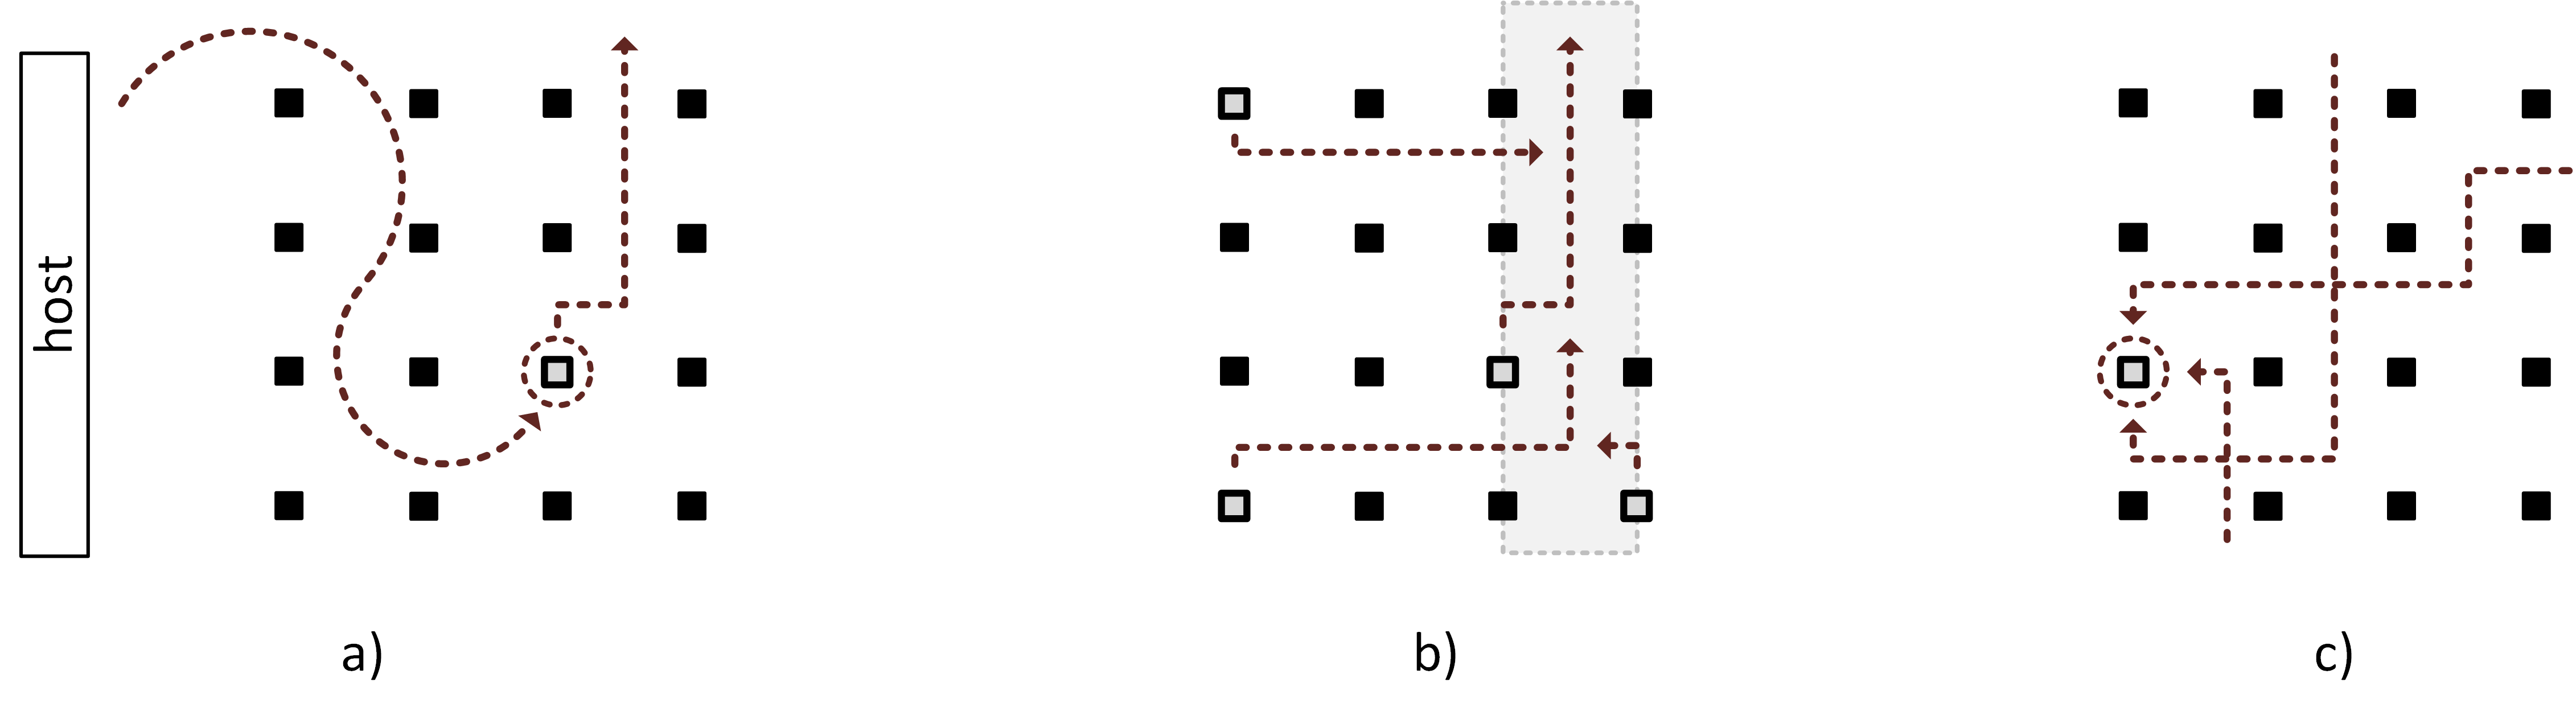
\includegraphics[scale=0.7]{figures/ch5_tradicional_net.png}
	\end{center}
	\caption
		{	
			Características en aceleradores convencionales. a) El procesamiento de información se lleva a cabo en un nodo específico de la red. b) Cada paquete portando el resultado de un proceso se dirige a una puerta de salida preestablecida, compitiendo con los recursos de transporte con los paquetes de recién ingreso al sistema. c) El uso de políticas desbalanceadas para la asignación de cargas de trabajo de un nodo puede saturar rápidamente varios canales de comunicación en el acelerador.
		}
	\label{fig:ch5_tradicional_net}
\end{figure}


La figura \ref{fig:ch5_propuesta_net} muestra la estructura propuesta para el acelerador conformado por múltiples núcleos de procesamiento. A grandes rasgos, este se encuentra compuesto por una red en-chip con topología malla, los nodos que pueblan la red pueden clasificarse dentro de 3 categorías: nodos frontera, nodos terminal y nodos centrales.

Cada clase de nodo se distingue por su capacidad de procesamiento y de direccionamiento de paquetes, a continuación se presenta una descripción de cada uno de ellos:

\begin{itemize}

	\item \textit{Nodo terminal:} Punto base para la inserción y captura de paquetes procesados por la red. Todo paquete que desee abandonar el acelerador, una vez que ha sido procesado, debe de dirigirse a uno de estos nodos para su extracción. Las terminales del acelerador deben estar colocadas en la periferia de la red, sin importar en cuál de sus frentes. Los nodos terminal cuentan con una unidad funcional, por lo que participan de manera activa en el procesamiento de paquetes. A nivel de micro-arquitectura los nodos terminal son equivalentes a un nodo central, sin embargo la implementación de su algoritmo de planificación de ruta difiere con estos últimos.

	\item \textit{Nodo central:} Elementos estándar de procesamiento. El interior de la red está formada por nodos centrales, los cuales cuentan con un elemento de procesamiento y la capacidad de encaminar paquetes a cualquiera de sus vecinos. El algoritmo de planificación de ruta de estos nodos no presenta alteración alguna, por lo que no tienen la capacidad de filtrar ningún tipo de paquete en tránsito. Todos los paquetes de nuevo ingreso son entregados a los nodos centrales a manos de los nodos frontera o terminal como se muestra en la figura \ref{fig:ch5_propuesta_net} c).

	\item \textit{Nodo frontera:} Los nodos frontera no contienen un elemento de procesamiento, por lo que no se consideran parte del área funcional de la red. Además de su falta de unidad funcional, su conectividad con la red se limita a un punto de captura e inyección de datos. Su tarea es la reinserción de paquetes que han alcanzado alguno de los límites de la red sin haber visitado una unidad funcional durante su trayecto, este comportamiento se muestra en la figura \ref{fig:ch5_propuesta_net} b).

\end{itemize}

\begin{figure}
	\begin{center}
		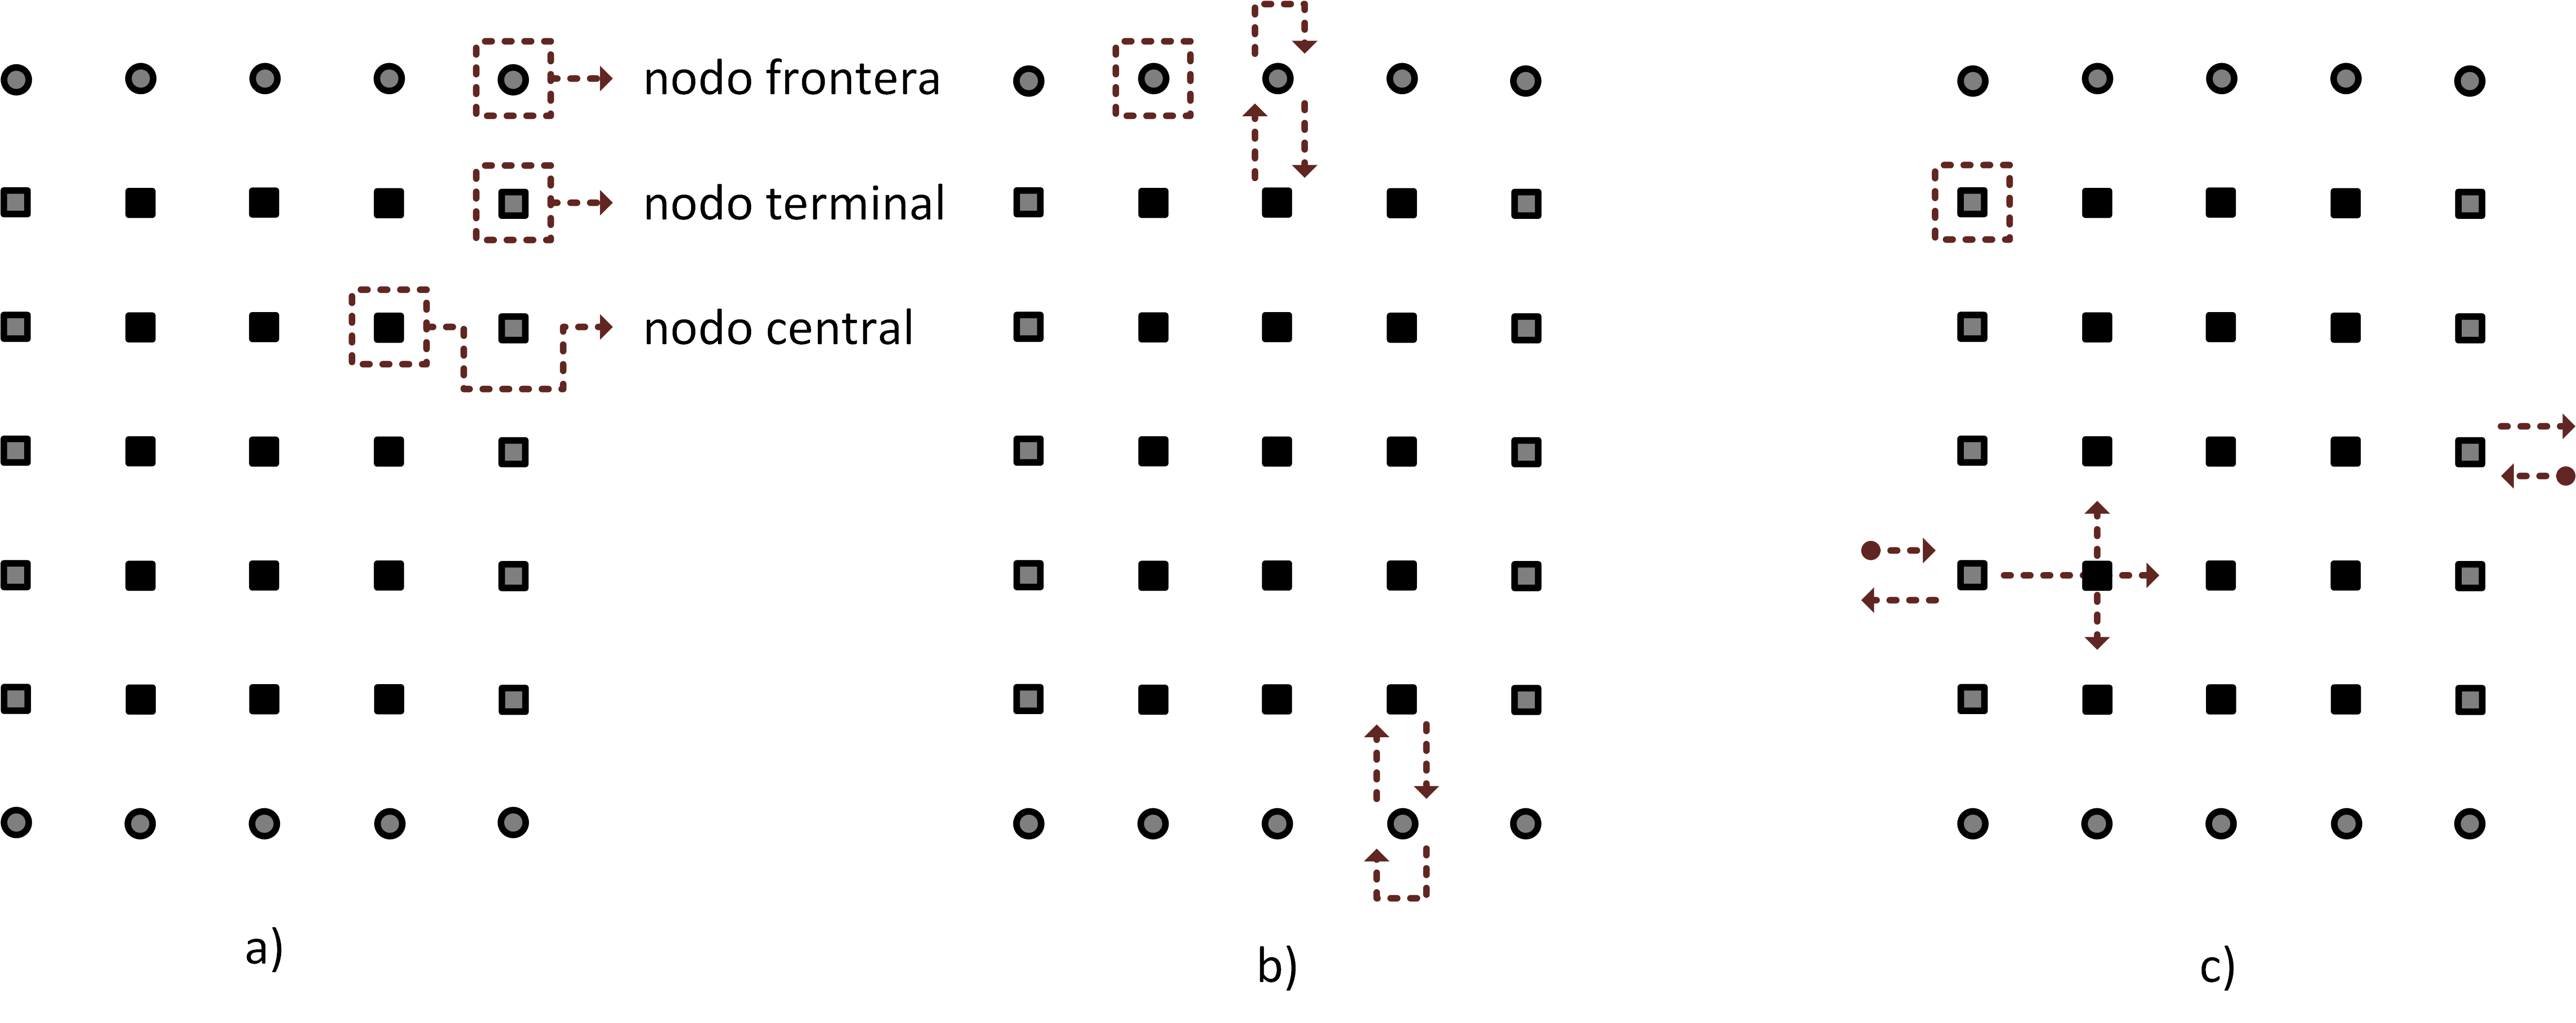
\includegraphics[scale=0.7]{figures/ch5_propuesta_net.png}
	\end{center}
	\caption
		{	
			Arquitectura propuesta. a) el acelerador está compuesto por una granja de núcleos comunicados por medio de una red en-chip, se hace uso de 3 tipos de nodo: Nodos terminales para la inyección y/o recepción de paquetes de la red, nodos frontera para re circular paquetes que no han sido procesados por una unidad funcional, y nodos centrales, los cuales procesan y envían los resultados fuera del acelerador. b) los nodos frontera solo tienen acceso a la red mediante un canal de comunicación. c) Los nodos terminal comparten micro-arquitectura con los nodos centrales, sin embargo, solo un nodo terminal es capaz de recibir y enviar paquetes fuera de la red.
		}
	\label{fig:ch5_propuesta_net}
\end{figure}

El procesamiento de un paquete en la arquitectura propuesta sigue el flujo de ejecución mostrado en la figura \ref{fig:ch5_transmision_paquete} y que se describe a continuación: un paquete ingresa a través de un nodo terminal en dirección a un nodo destino. La cabecera de cada paquete contiene una dirección destino y una dirección de puerta de salida, los campos que conforman la cabecera de un paquete puede encontrarse en el capitulo \ref{chap:nodo_de_red} dentro de la sección \ref{subsec:formato_de_paquete}. El paquete en tránsito busca llegar a la dirección destino asignada en su flit de cabecera, todas las direcciones destino corresponden a nodos frontera. Durante su avance a través de la red, el paquete busca un nodo cuya unidad funcional se encuentre disponible para el procesamiento de la información que acarrea consigo. En caso de llegar a un nodo atendiendo una petición previa, el paquete seguirá adelante como se muestra en la figura \ref{fig:ch5_transmision_paquete} a). Al alcanzar un nodo frontera, el paquete ingresa para la asignación de un nuevo nodo destino y su posterior reenvío a la red en búsqueda de una unidad de procesamiento disponible. Al encontrar un nodo disponible para el procesamiento de información, el paquete lleva a cabo una solicitud de ingreso. Una vez finalizado el procesamiento de información dentro de la unidad funcional, la cabecera del paquete cambia su dirección destino por la dirección del nodo terminal donde está programada su salida de la red. 

El uso de una estrategia \textit{el primero en llegar, el primero en ser atendido} para la asignación de recursos de procesamiento libera la presión sobre nodos específicos de la red, permitiendo un continuo flujo de paquetes a través del sistema. Para implementar la estrategia descrita anteriormente es necesario el uso de un nuevo esquema de planificación de ruta a través de la red. Como se mencionó en el capitulo \ref{chap:fundamentos}, dentro de la sección \ref{sec:conceptos_basicos_de_nocs}, los algoritmos de planificación de ruta tradicionales requieren de un destino fijo para el manejo de paquetes, una vez alcanzado dicho destino el paquete lleva a cabo una solicitud de ingreso al elemento de procesamiento del nodo actual. El acelerador basado en múltiples núcleos de este trabajo agrega como primera opción de ruta el elemento de procesamiento de cualquier nodo visitado, en caso de no estar disponible, el algoritmo se comportara de manera tradicional y solicitara el uso del puerto de salida que lo aproxime a su destino.

El algoritmo de planificación de ruta requiere de un mecanismo externo para mantener la circulación de paquetes de manera continua a través de todos los nodos de la red, este mecanismo externo se implementa por medio de los nodos frontera del acelerador. Los nodos frontera no pueden llevar a cabo ninguna tarea de procesamiento y su micro arquitectura difiere en gran medida con la de los demás módulos de la red. Internamente los nodos frontera no implementan mecanismo de arbitraje entre puerto debido a que todo paquete ingresando solo tiene la posibilidad de egresar por un solo canal. El mecanismo de control de flujo si se encuentra implementado en estos nodos para mantener el protocolo de intercambio de información a nivel de capa física con los demás bloques del acelerador. 

\begin{figure}
	\begin{center}
		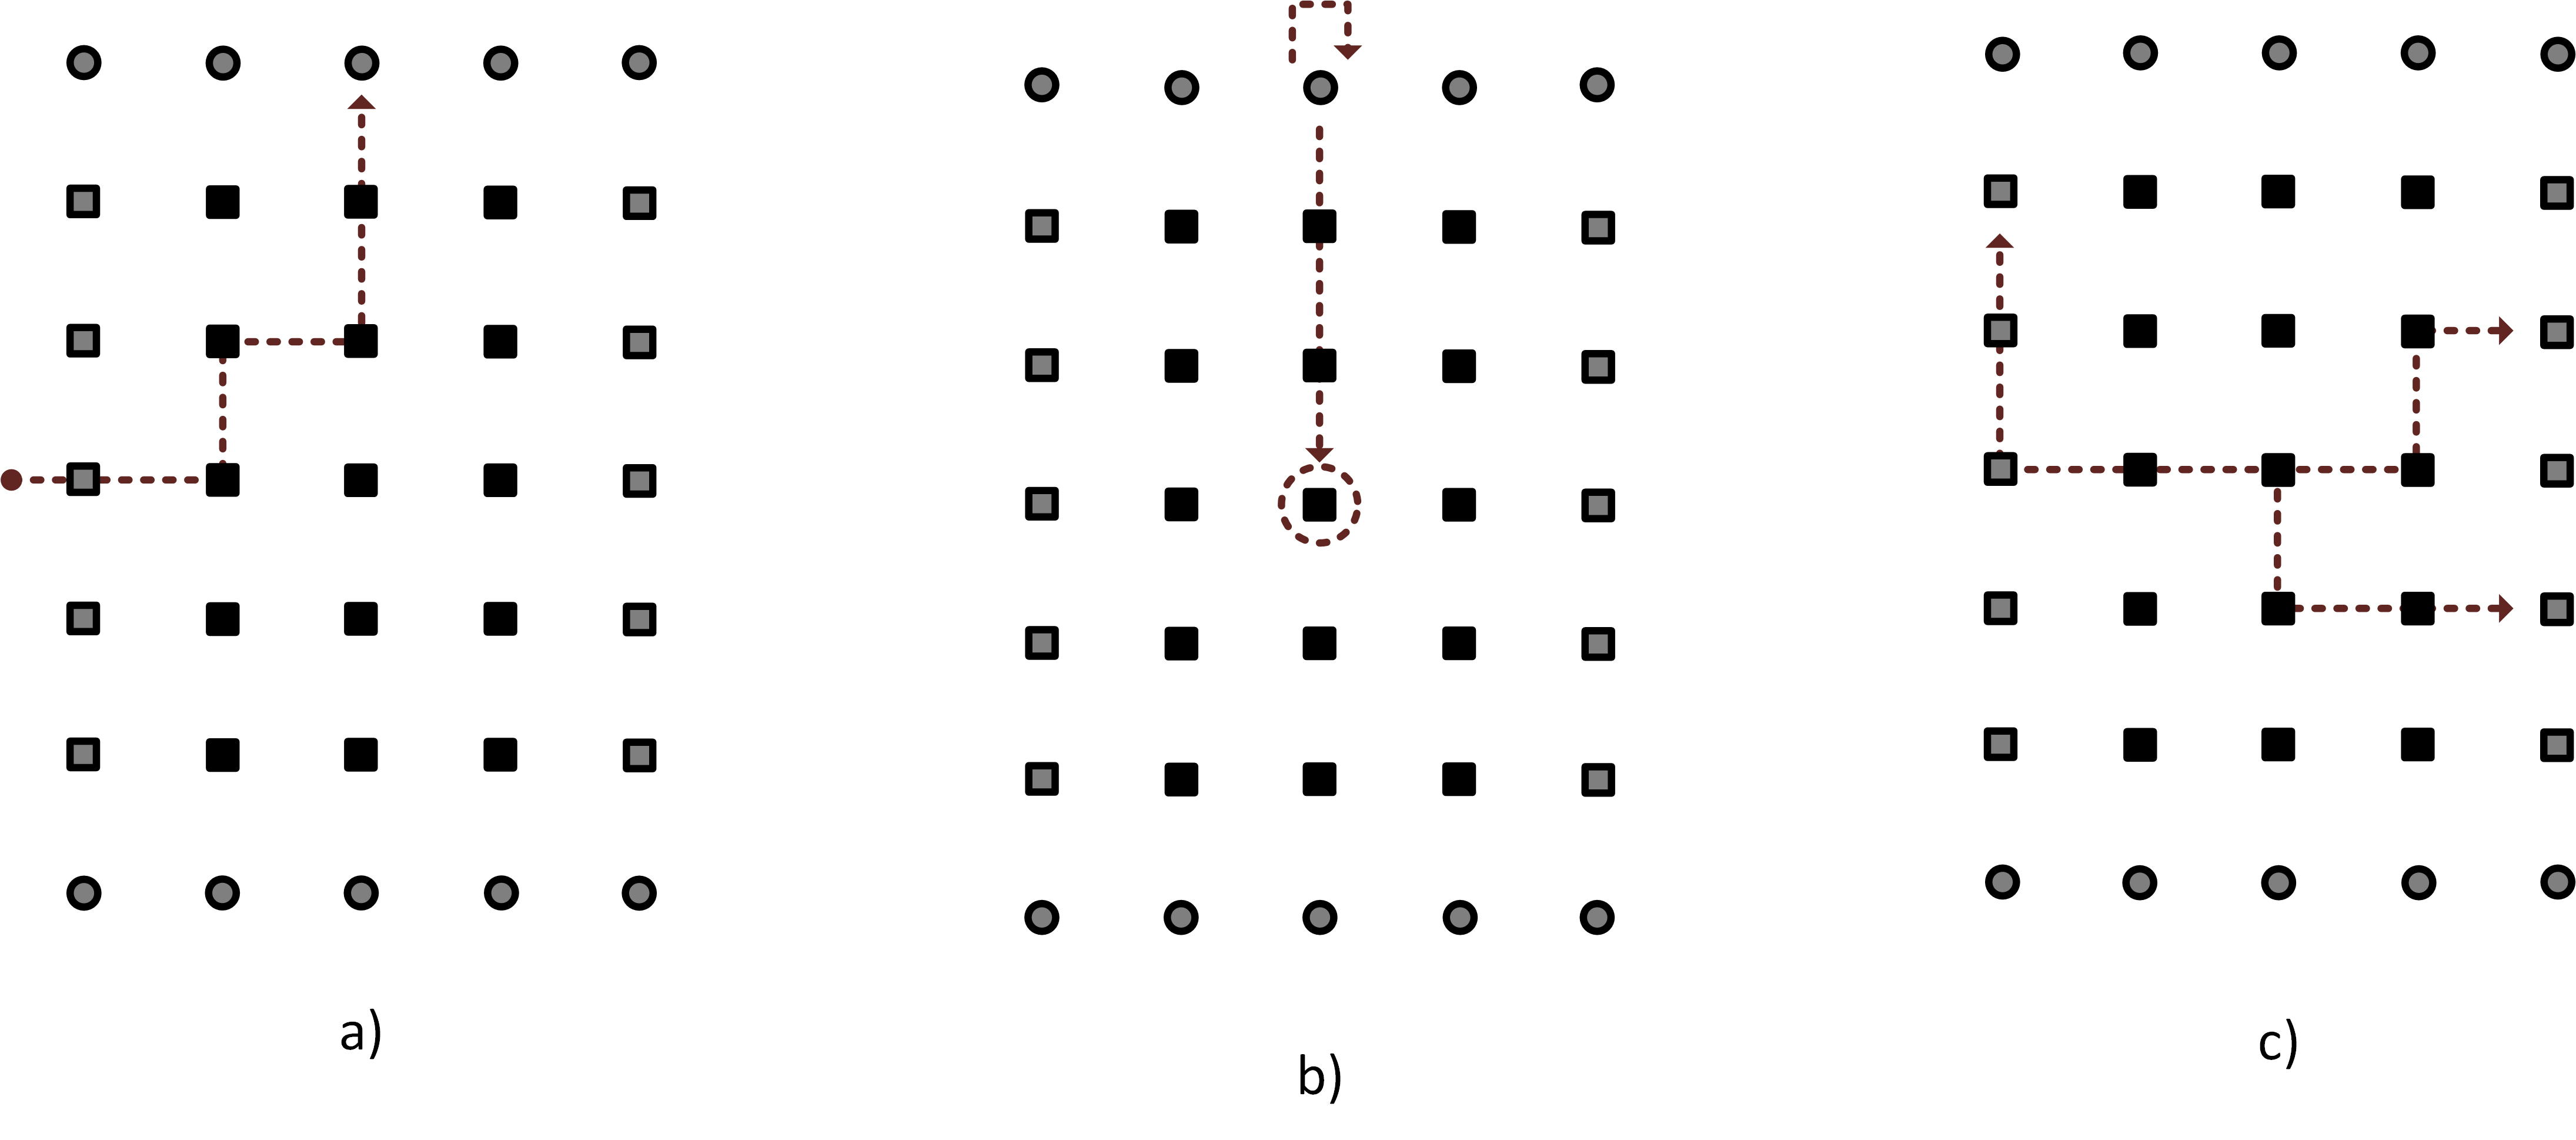
\includegraphics[scale=0.7]{figures/ch5_transmision_paquete.png}
	\end{center}
	\caption
		{	
			Tránsito de un paquete a través del acelerador. a) en primera instancia un paquete ingresa a través de un nodo terminal. El paquete buscará la primera unidad funcional disponible para el procesamiento de información. b) en caso de alcanzar un nodo frontera sin haber procesado su información, el paquete cambia su dirección y continúa la búsqueda de una unidad funcional disponible. c) Una vez terminado el procesamiento de información de un paquete, este reingresa a la red en búsqueda de un nodo terminal para su egreso del sistema.
		}
	\label{fig:ch5_transmision_paquete}
\end{figure}

La estrategia de distribución de carga de trabajo, en conjunto con el medio de reinserción de paquetes no procesados a la red, forman el mecanismo híbrido en el cual se basa el acelerador presentado en este trabajo.


\section{Módulos propios del acelerador multi-núcleo}
	\label{sec:ch5_modulos_propios_del_acelerador}

El sistema de navegación de paquetes a través de la red está dividido en dos partes: en primer lugar se encuentra el algoritmo modificado de encaminamiento, el cual se encuentra distribuido a través de todos los nodos del sistema. Cualquier algoritmo de encaminamiento que no requiera de canales virtuales y sea viable para trabajar sobre redes de topología malla puede adecuarse para trabajar en la arquitectura propuesta.

En segundo lugar, se encuentra el mecanismo re inserción de paquetes a la red, el cual es implementado por medio de nodos frontera. La decisión del uso de módulos dedicados para llevar a cabo esta función se tomó en aras de mantener un diseño sencillo de los nodos de procesamiento de la red. La implementación de esta restricción extra como una característica más del algoritmo de encaminamiento aumentaría el grado de complejidad de todo el sistema.

En esta sección se presenta la arquitectura de los nodos frontera así como una descripción de su participación en el flujo de información a través del acelerador. En segundo lugar se presenta la metodología desarrollada para la modificación de algoritmos de encaminamiento pre existentes. La figura \ref{fig:ch5_direccionamiento} a) muestra el esquema de etiquetado de nodos de la red, este se utilizara en los ejemplos de esta sección.


\subsection{Nodo Frontera}
	\label{subsec:ch5_nodo_frontera}

La figura \ref{fig:ch5_nodo_frontera} muestra la arquitectura interna de nodo frontera de la red. La tarea a llevar por estos módulos es el proporcionar un punto inicial de destino para todos los paquetes ingresando a la red. Los paquetes buscan llegar a su punto destino, sin embargo, harán la solicitud de ingreso a una unidad funcional disponible en cualquiera de los nodos que se visite en su trayecto. Un paquete procesado cambia su dirección destino por una dirección de salida de la red.

Todos los paquetes que no encontraron en su camino un procesador disponible eventualmente alcanzan un nodo frontera. El nodo frontera al recibir el paquete modificara la dirección destino por la dirección de un nodo frontera opuesto a el y posteriormente reenviará el paquete para que continúe su búsqueda de un procesador en una dirección distinta. 

\begin{figure}
	\begin{center}
		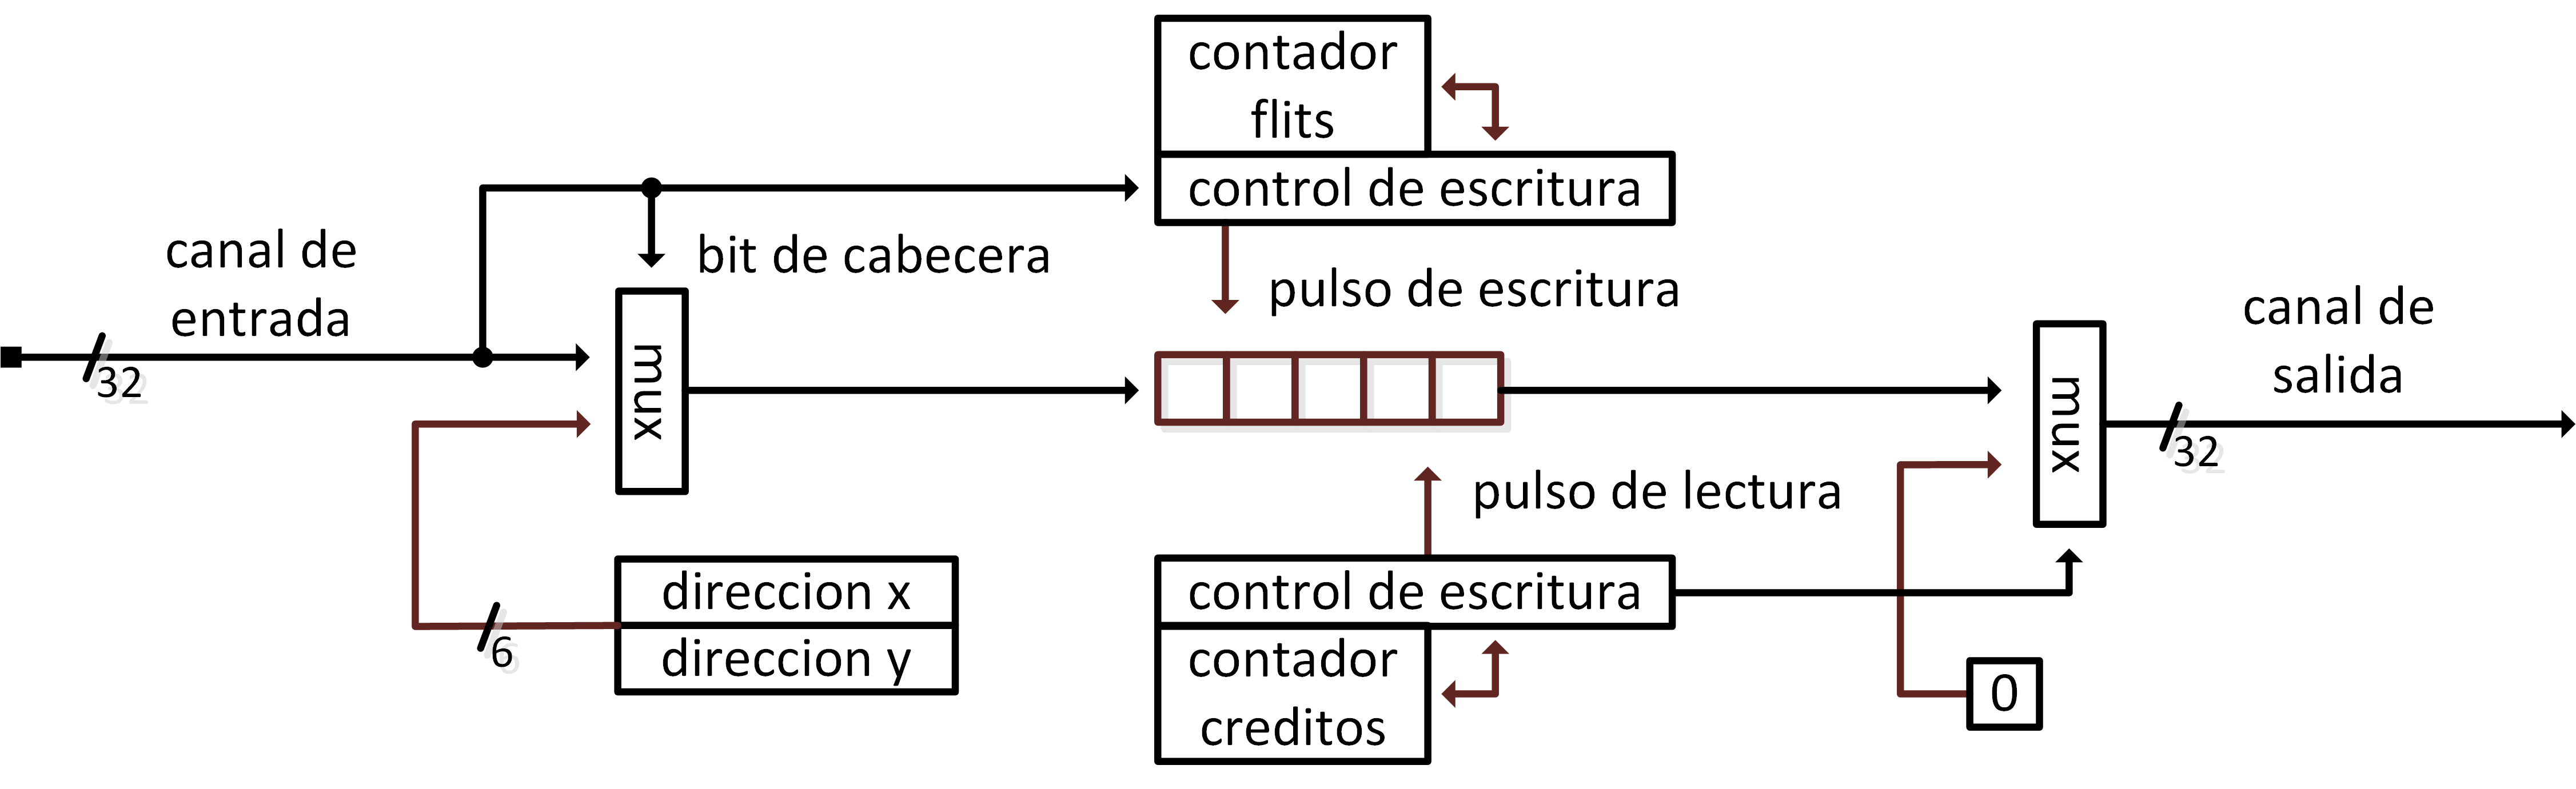
\includegraphics[scale=0.7]{figures/ch5_nodo_frontera.png}
	\end{center}
	\caption
		{	
			Arquitectura de nodo frontera. El camino de datos de este módulo solo lleva a cabo la sustitución de la dirección destino de los paquetes en tránsito.
		}
	\label{fig:ch5_nodo_frontera}
\end{figure}

Internamente el nodo frontera está formado por una estructura \textit{FIFO} de almacenamiento temporal y dos máquinas de estado independientes que se encargan del ingreso y egreso de paquetes a la red. El control de flujo de datos dentro de un nodo frontera se lleva a cabo de mediante un contador de créditos, de esta manera se homologa el flujo de datos con todos los otros nodos de la red.

Las máquinas de estado siguen la misma lógica de captura y liberación que se presenta en los módulos MEFE y MEFS de la arquitectura del encaminador, esta se puede consultar en el capitulo \ref{chap:nodo_de_red} dentro de la sección \ref{puerto_entrada}. Los nodos frontera requieren de una dirección estática que se asignará a todos los paquetes rebotando a la red a través de ellos, esta dirección se determina de manera previa a la síntesis del sistema y debe de cumplir con las restricciones impuestas por el algoritmo de enrutamiento, de lo contrario existe el riesgo de crear \textit{deadlocks} o \textit{livelocks} en la red.

La sobre escritura de la dirección destino de un paquete se lleva a cabo durante el ingreso del flit de cabecera al \textit{FIFO} del nodo, evitando la necesidad de lógica extra durante la salida del paquete. La figura \ref{fig:ch5_direccionamiento} b) muestra un acelerador utilizando el algoritmo de encaminamiento \textit{west first minimal}. 


\subsection{Modulo Planificador de Ruta}
	\label{subsec:ch5_modulo_planificador_de_ruta}

La capacidad de los paquetes para ingresar a cualquier núcleo de procesamiento de la red radica en el algoritmo de encaminamiento de información. La inserción del mecanismo de solicitud de ingreso a elementos de procesamiento en cada salto de un paquete es implementado mediante la alteración de un algoritmo pre existente, sin embargo, para mantener el continuo flujo de información se requiere la integración de nodos frontera.

A grandes rasgos, el proceso de modificación de un algoritmo de encaminamiento pre existente consiste en la inserción de un nivel jerárquico superior, en donde la solicitud de entrada a un elemento de procesamiento tenga un nivel mayor de prioridad respecto al orden propuesto por el algoritmo original. De igual forma, se debe de incluir un supresor de la modificación en el algoritmo en caso de que el paquete en circulación ostente una bandera indicando que ya a sido procesado en un nodo anterior.

El algoritmo de encaminamiento original tiene un fuerte impacto en el cálculo de las direcciones válidas a las que un nodo frontera puede redirigir su tráfico. La figura \ref{fig:ch5_direccionamiento} b) muestra una red hipotética utilizando el algoritmo de encaminamiento \textit{west first minimal}, el cual se discutió en el capitulo \ref{ch:topicos_selectos} sección \ref{subsec:algoritmo_west_first_minimal}, este algoritmo prohíbe giros en la dirección \textit{x-}, por lo que paquetes saliendo de los nodos frontera con dirección a nodos terminales o centrales que se encuentren a la izquierda de los mismos producen el riesgo de crear deadlocks como se muestra en la misma figura. De manera general el proceso de modificación de un algoritmo de encaminamiento requiere analizar las rutas y direcciones válidas para los nodos frontera de la red.

\begin{figure}
	\begin{center}
		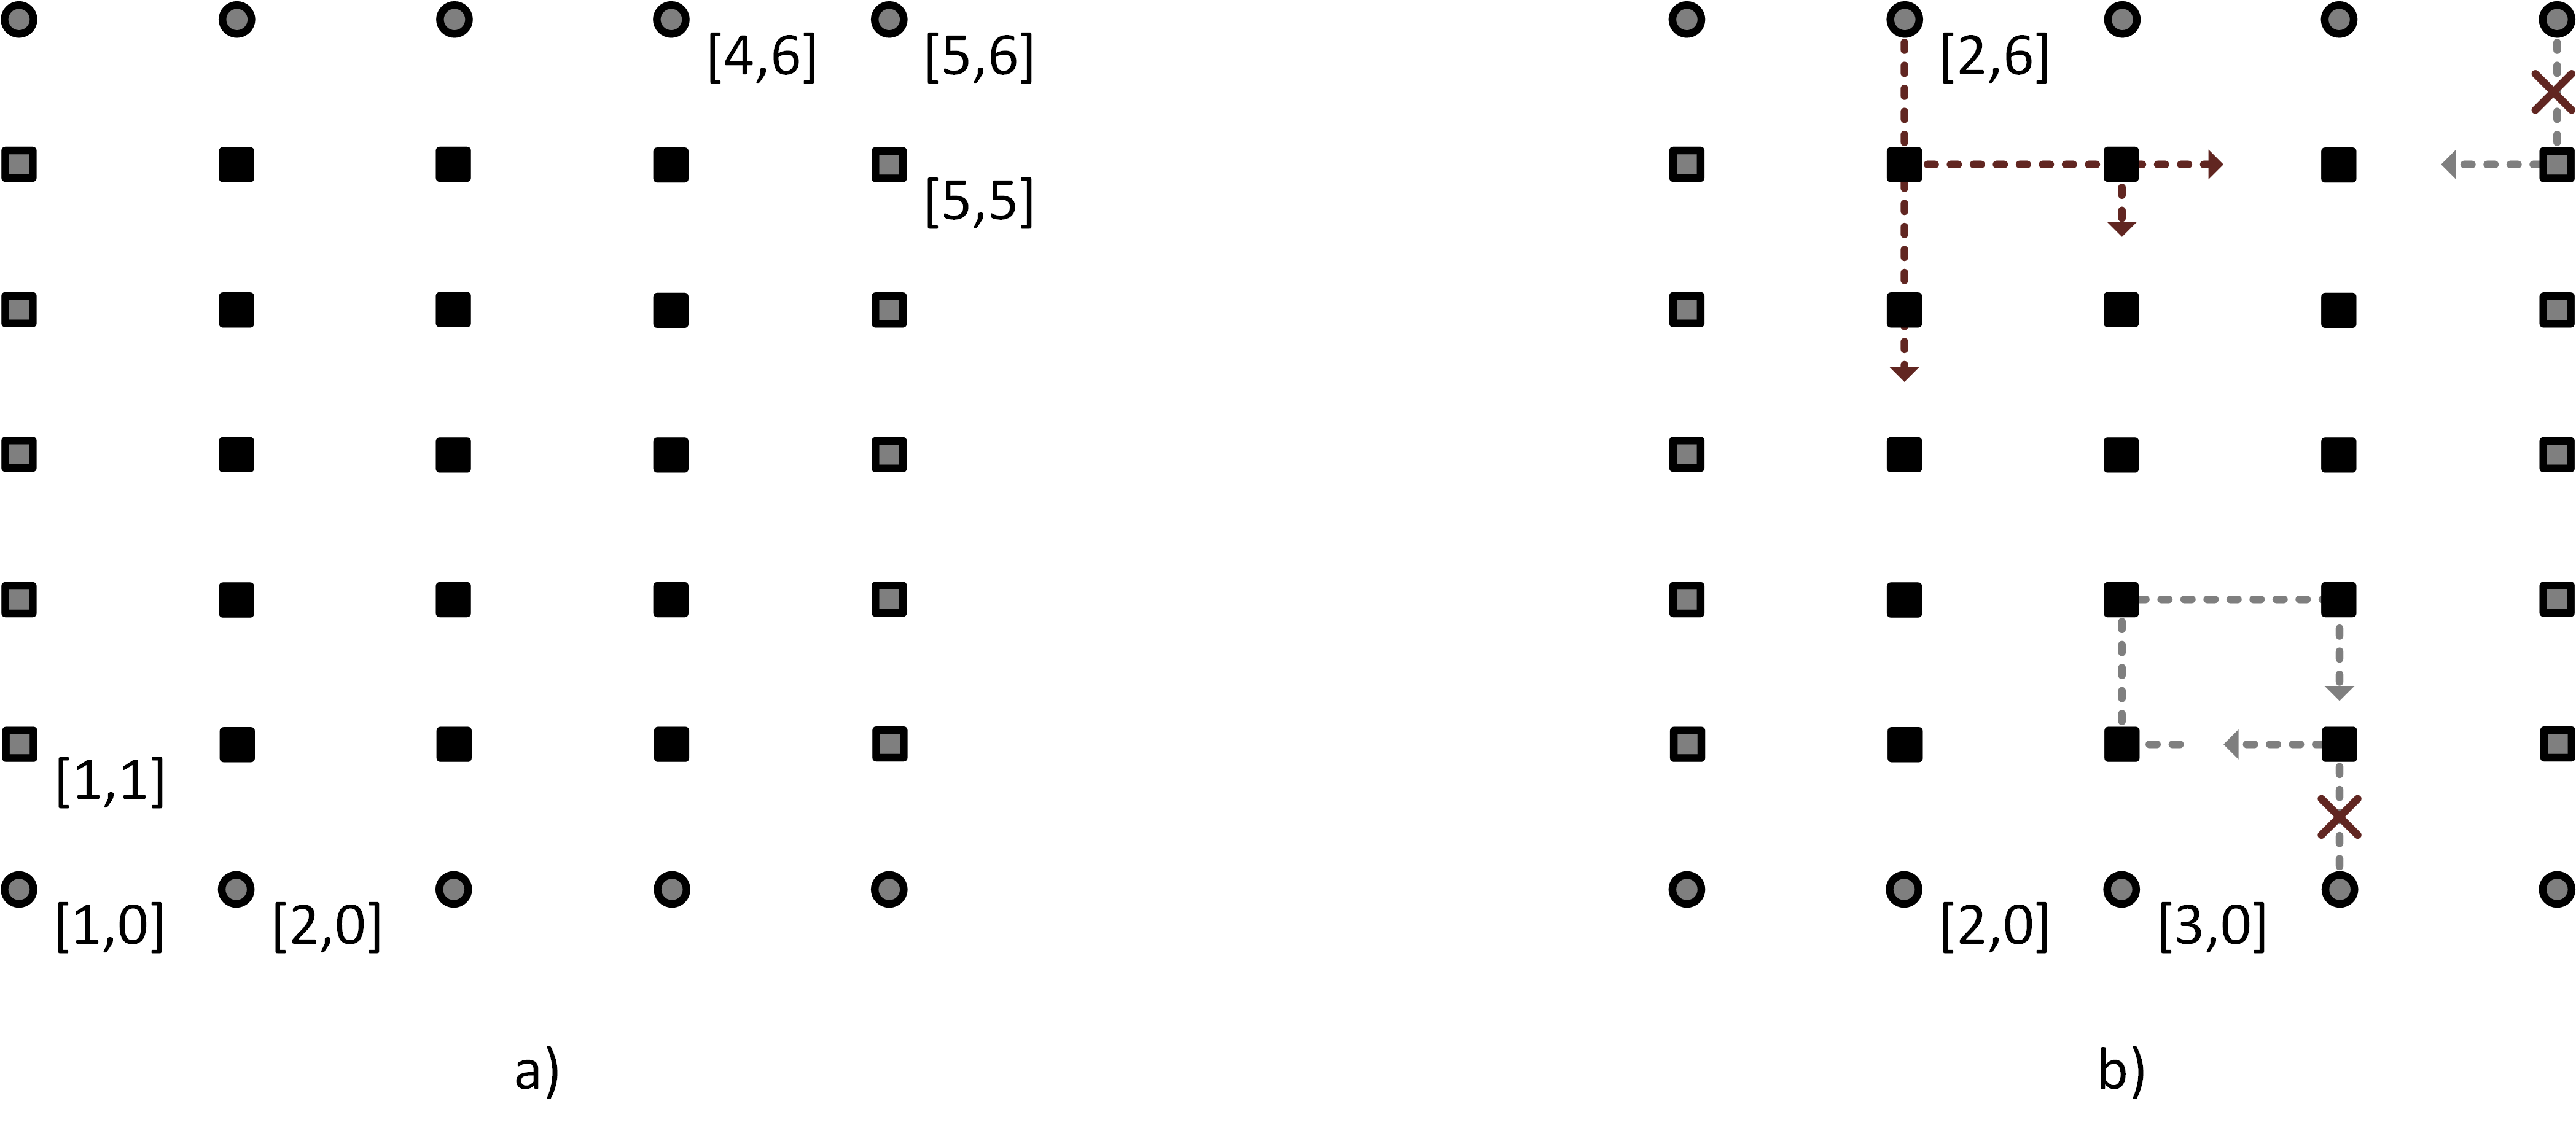
\includegraphics[scale=0.6]{figures/ch5_direccionamiento.png}
	\end{center}
	\caption
		{	
			a) Los nodos se etiquetan de acuerdo a su posición en la red. Vale la pena notar que todos los nodos centrales formarán una sub-red tipo malla al centro del acelerador. Las etiquetas para cada nodo sirven para reconocer que trabajo desempeña en el acelerador, además de facilitar la selección de instancia correcta durante el proceso de síntesis del sistema. b) Los nodos frontera deben de tomar en cuenta las restricciones impuestas por el algoritmo de encaminamiento para la selección de direcciones válidas en sus paquetes de salida.
		}
	\label{fig:ch5_direccionamiento}
\end{figure}

La modificación de un algoritmo de encaminamiento pre existente requiere realizar un cambio en la estructura jerárquica de selección de puerto de salida. Dentro de la estructura de selección de puerto, se inserta en el nivel superior la solicitud de ingreso a el elemento de procesamiento si y sólo si el paquete contiene la información original en sus flits de datos. En caso de que el campo de \textit{testigo de post - proceso} presente un estado alto, esta solicitud se omite y se continúa con el árbol de selección de siguiente salto para el paquete. El código \ref{code:west_first_minimal_extended} muestra la modificación pertinente para el algoritmo \textit{West First Minimal} que se mostró en el capitulo \ref{ch:topicos_selectos} dentro de la sección \ref{subsec:algoritmo_west_first_minimal}.


\begin{algorithm}[]
	\KwData{dirección de nodo actual  (\textit{localX}, \textit{localY})}
	\KwData{dirección de nodo destino (\textit{destX},  \textit{destY} )}
	\KwData{campo de testigo de procesamiento}		
	\KwResult{canales de salida válidos (\textit{canales})}
		\Begin
			{
			offsetX = destX - localX\;
			offsetY = destY - localY\;
				\If{campo de testigo de procesamiento}
					{
						canales := elemento de procesamiento\;
					}
				\If{offsetX < 0}
					{
						canales := X-\;
					}
				\If{offsetX > 0 \textbf{and} offsetY < 0}
					{
						canales := (X+, Y-)\;
					}
				\If{offsetX > 0 \textbf{and} offsetY > 0}
					{
						canales := (X+, Y+)\;
					}
				\If{offsetX > 0 \textbf{and} offsetY = 0}
					{
						canales := X+\;
					}
				\If{offsetX = 0 \textbf{and} offsetY < 0}
					{
						canales := Y-\;
					}
				\If{offsetX = 0 \textbf{and} offsetY > 0}
					{
						canales := Y+\;
					}
		}
	\caption
		{
			\textit{West-First minimal} para nodos centrales del acelerador.
		}	
	\label{code:west_first_minimal_extended}
\end{algorithm}

El código \ref{code:west_first_minimal_extended} es utilizado de manera exclusiva en nodos centrales de la red, ya que no cuenta con un mecanismo para manejar el caso en el cual la dirección local del nodo es la dirección destino del paquete. Este caso se omite debido a que el diseño de la red prohíbe se asigne un nodo central como destino de un paquete. La versión del algoritmo para nodos terminales requiere el manejo del escenario anterior, donde el nodo terminal destino retira de la red el paquete recibido.

\begin{figure}
	\begin{center}
		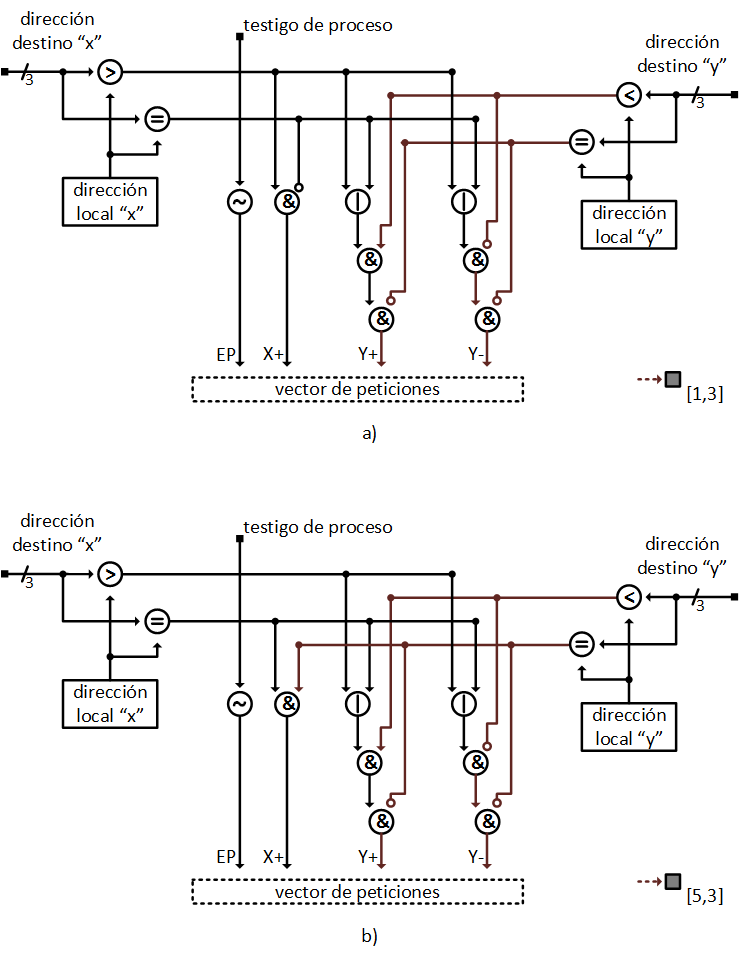
\includegraphics[scale=0.75]{figures/ch5_segmento_wfm.png}
	\end{center}
	\caption
		{	
			a) Módulo planificador de ruta para puerto \textit{x-} del nodo [1,3]. b) Módulo planificador de ruta para puerto \textit{x-} del nodo [5,3], el nodo en cuestión maneja la salida de red a través del puerto \textit{x+}.
		}
	\label{fig:ch5_segmento_wfm}
\end{figure}

La implementación en hardware de este algoritmo no se lleva de manera centralizada, es decir, no existe un módulo centralizado de calculo de ruta para todos los paquetes llegando al router. En su lugar, se distribuye el cálculo de ruta entre los diferentes puertos de entrada, donde cada uno de ellos integra un segmento del algoritmo que atiende solo los casos que se pueden presentar para los paquetes ingresando desde esa dirección. La figura \ref{fig:ch5_segmento_wfm} en sus apartados a) y b), muestra el diagrama de los segmentos del algoritmo implementado en los puertos de entrada \textit{x-} de los nodos terminal (5,3) y (1,3). Se puede apreciar la diferencia del hardware generado para cada instancia. El segmento de algoritmo mostrado en el código \ref{code:west_first_minimal_terminal} representa el segmento para el envío de paquetes fuera de la red.


\begin{algorithm}[]
		\Begin
			{
				\If{offsetX == 0 \textbf{and} offsetY == 0}
					{
						canales := X-\;
					}
			}
	\caption
		{
			Condicional exclusiva para nodos terminal del acelerador.
		}	
	\label{code:west_first_minimal_terminal}
\end{algorithm}


Es necesario recordar que el algoritmo \textit{west first minimal} es parcialmente adaptativo, por lo que ofrece múltiples opciones de puertos de salida en caso que varias direcciones acerquen al paquete a su destino. La salida de los segmentos presentados en la figura \ref{fig:ch5_segmento_wfm} requieren una conexión a un módulo SP descrito en el capitulo \ref{chap:nodo_de_red} dentro de la sección \ref{puerto_entrada}. La adaptación de algoritmos no adaptativos conlleva el mismo procedimiento descrito anteriormente para su incorporación al acelerador propuesto, el código \ref{code:xy_extended} muestra una versión modificada del algoritmo \textit{XY} para el uso dentro del acelerador.

La figura \ref{fig:ch5_segmento_xy} muestra el segmento de selección de ruta para el próximo salto en la red mediante el uso del algoritmo \textit{XY}. La metodología para extender el uso de algoritmos no adaptativos sigue la misma directriz de agregar un nivel jerárquico en la toma de decisiones de la ruta a seguir.

\begin{figure}
	\begin{center}
		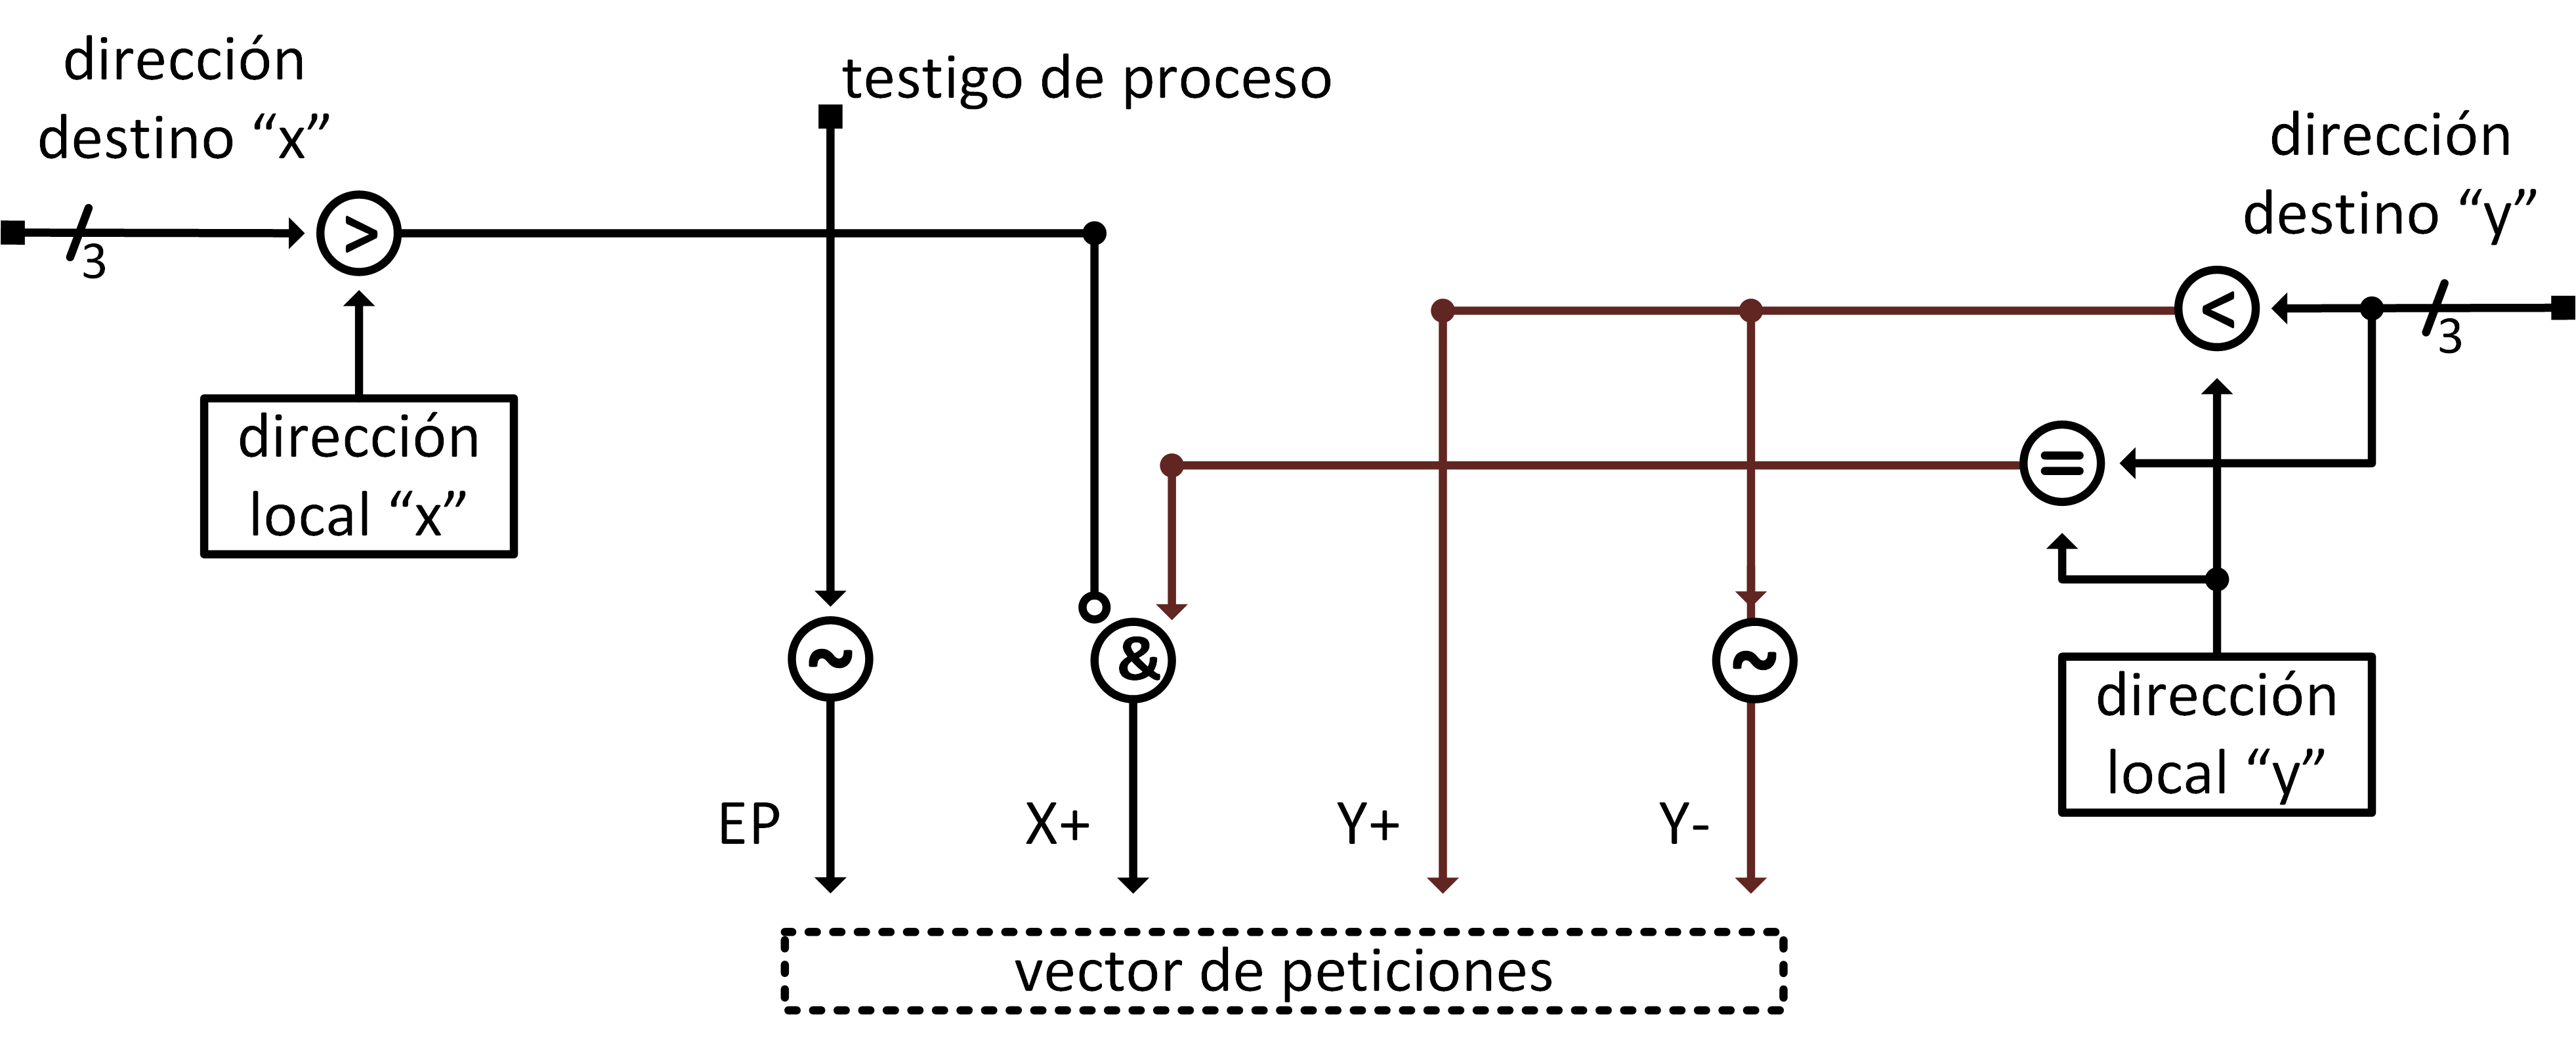
\includegraphics[scale=0.75]{figures/ch5_segmento_xy.png}
	\end{center}
	\caption
		{	
			Segmento de calculo de ruta en el puerto de entrada \textit{x-} mediante el uso del algoritmo \textit{XY}.
		}
	\label{fig:ch5_segmento_xy}
\end{figure}


\begin{algorithm}[]
	\KwData{dirección de nodo actual  (\textit{localX}, \textit{localY})}
	\KwData{dirección de nodo destino (\textit{destX},  \textit{destY} )}
	\KwData{campo de testigo de procesamiento}		
	\KwResult{canales de salida válidos (\textit{canales})}
		\Begin
			{
			offsetX = destX - localX\;
			offsetY = destY - localY\;
				\eIf{testigo de procesamiento}
					{canal := elemento de procesamiento\;}
					{
						\eIf{offsetX > 0}
							{canal := X+\;}
							{
								\eIf{offsetX < 0}
									{canal := X-\;}
									{
										\eIf{offsetY > 0}
											{canal := Y+\;}
											{canal := Y-\;}
									}
							}
					}			
		}
	\caption
		{
			Algoritmo \textit{XY} modificado para su uso en la arquitectura de acelerador propuesta.
		}	
	\label{code:xy_extended}
\end{algorithm}



\section{Andamiaje de validación}
	\label{ch5_andamieje_de_validacion}

La validación del acelerador se llevó a cabo de manera progresiva, donde cada bloque se somete a pruebas funcionales. Los sub-módulos del sistema utilizan camas de prueba sencillas para su evaluación, estas se pueden encontrar en el repositorio del proyecto (\url{github.com/hcabrera-/lancetfish/}) dentro de los directorios \textit{verif}.

La evaluación del acelerador a nivel sistema se llevó a cabo mediante el módulo denominado \textit{network core}, este último está formado por el arreglo de nodos en topología tipo malla, junto a sus respectivos canales de interconexión. Cada nodo se enlaza con sus vecinos mediante un canal de transmisión y uno de recepción. Los canales están compuestos por un bus de 32 bits para la transmisión de datos, una línea de señalización para el envío o recepción de créditos y un par diferencial para el control de flujo entre nodos. El núcleo estándar de red para las pruebas funcionales está compuesto por 10 nodos terminal, 15 nodos centrales y 10 nodos frontera como se muestra en la figura \ref{fig:ch5_organizacion_validacion}.

Para la inyección y captura de paquetes se desarrollaron los módulos de verificación \textit{source} y \textit{sink}, ambos descritos a nivel comportamental. Los módulos de verificación ofrecen un conjunto de métodos y atributos para interactuar con la red así como para la captura de resultados.
Cada canal de entrada del módulo \textit{network core} se conecta a un módulo \textit{source}, mientras cada canal de salida será enlazado con un módulo sink.

El módulo \textit{source} provee 4 servicios principales: recepción de créditos de manera automática, este es un servicio que no requiere ser invocado y se encuentra en ejecución en segundo plano desde el inicio de la simulación. Envío de paquetes mediante la tarea \textit{send packet}, este método se encarga de la deconstrucción de una cada dena de datos para su envío en flits, además de mantener los protocolos de control de flujo de datos utilizado por la red. La tarea \textit{send packet} requiere se proporcione una cadena de bits que contenga la información que conforma un paquete. Los dos métodos restantes del módulo se encarga de la apertura y cierre de bitácoras de eventos para el módulo.

Es importante notar que el módulo source no tiene manera de generar paquetes válidos para la red, su tarea se limita al control físico del envío de datos. Para cumplir esta tarea se proporciona el módulo \textit{packet generator}, el cual se describe más adelante en esta sección.

\begin{figure}
	\begin{center}
		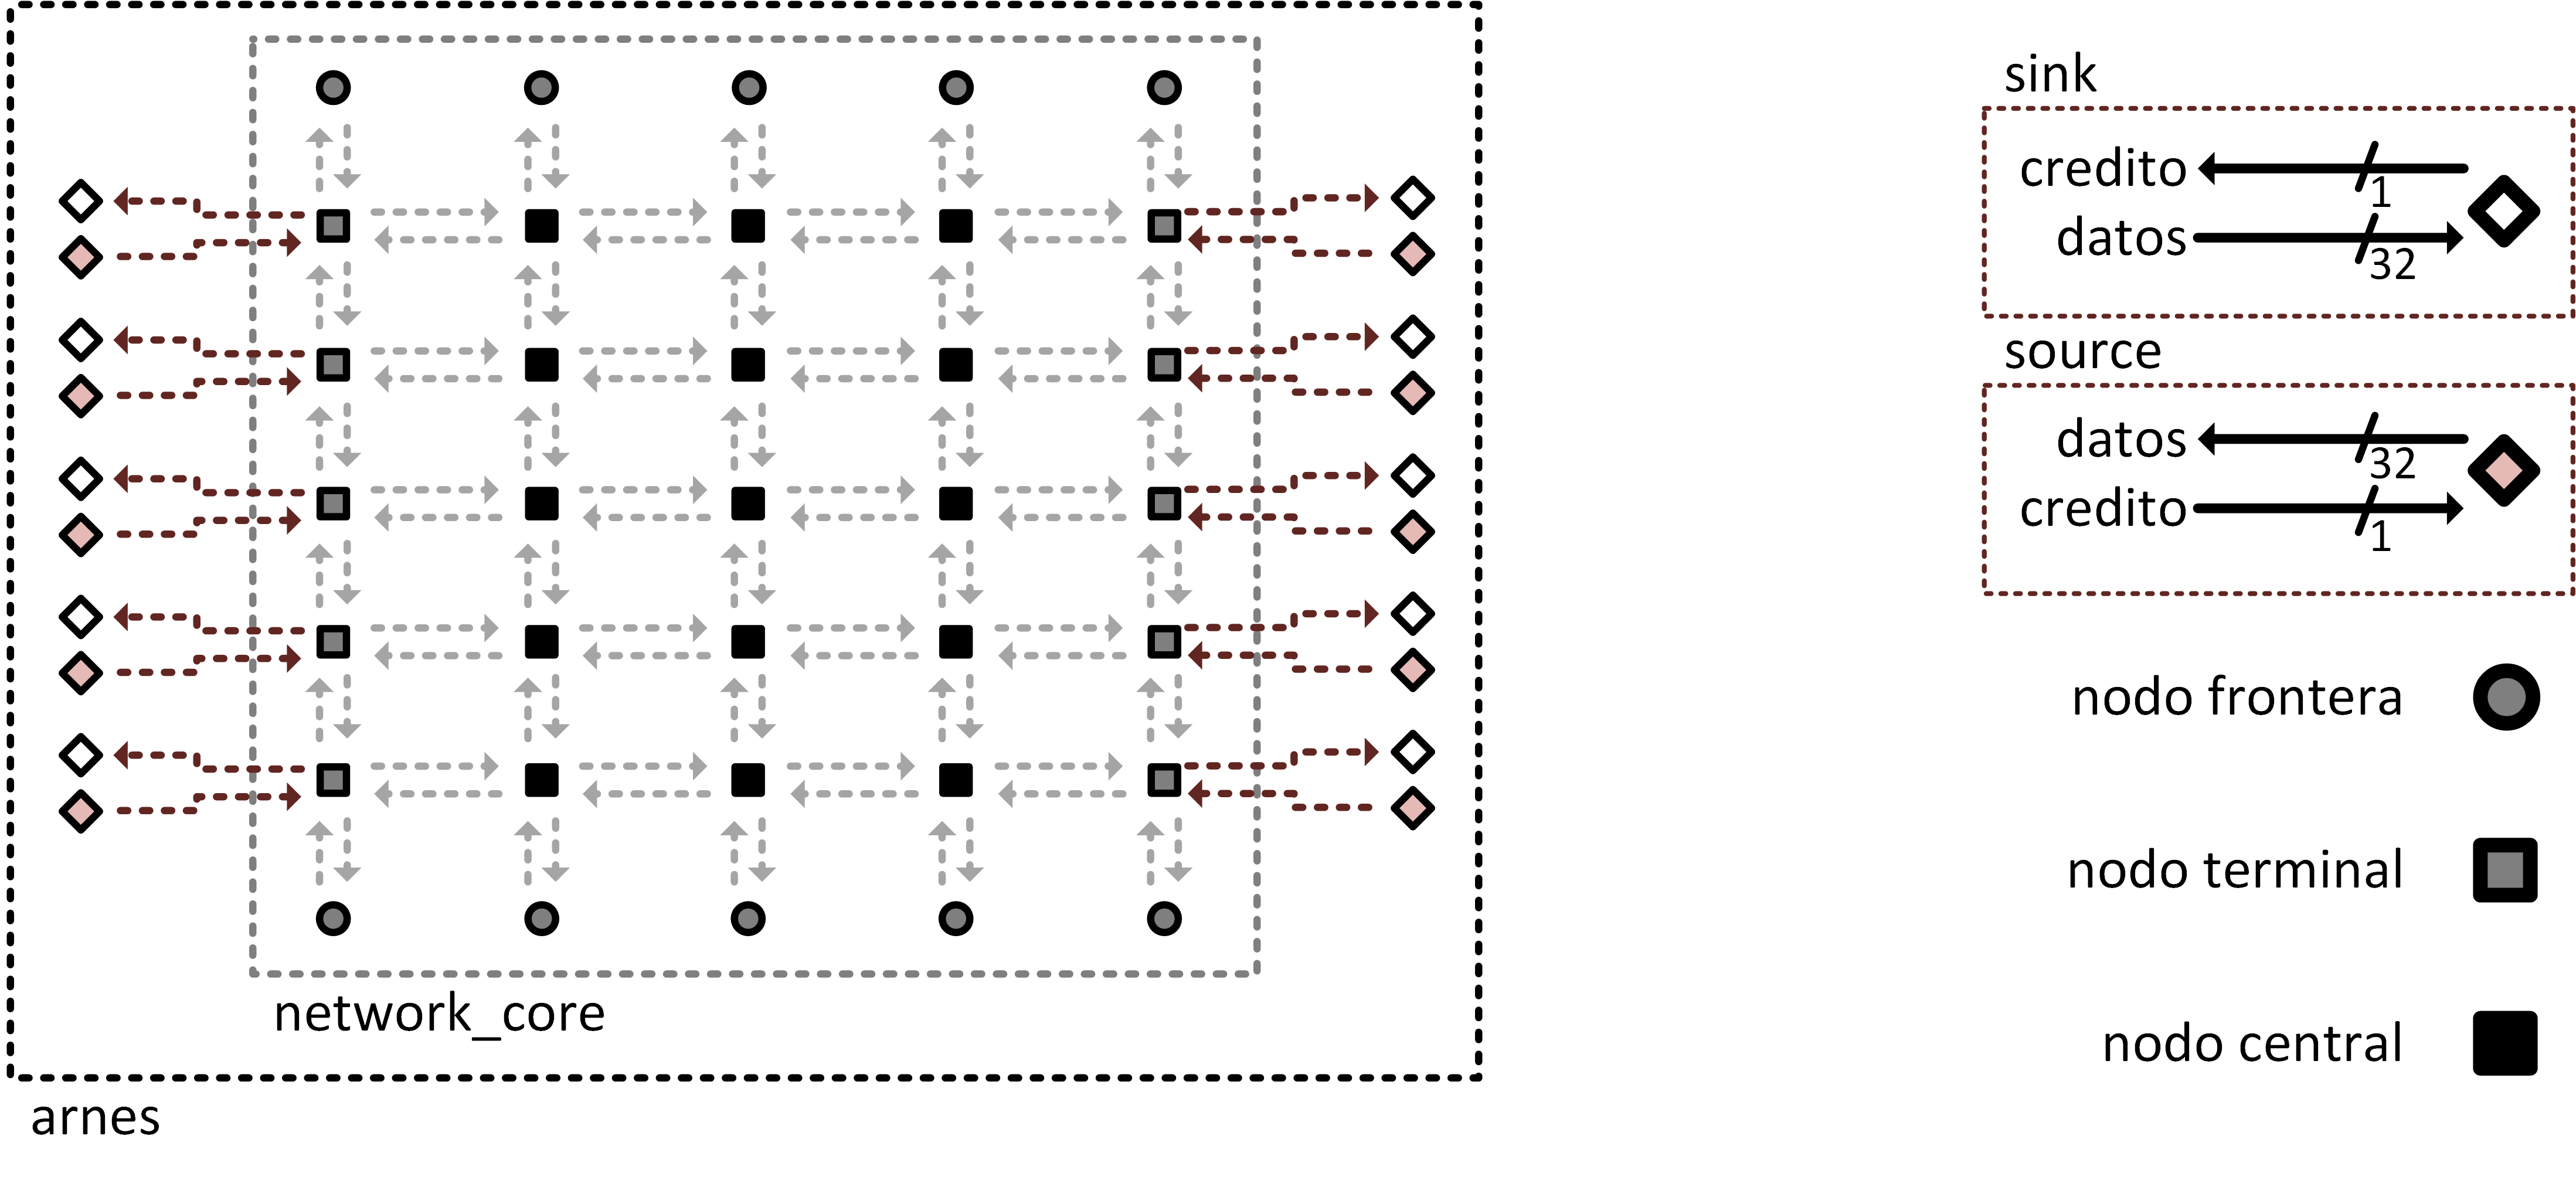
\includegraphics[scale=0.75]{figures/ch5_organizacion_validacion.png}
	\end{center}
	\caption
		{	
			El núcleo de la red integra todos los nodos necesarios para su funcionamiento, sin embargo no incluye un mecanismo para la inyección de paquetes. El arnés provee de los medios para evaluar el núcleo de la red, incluyendo medios para el envió y recepción de paquetes.
		}
	\label{fig:ch5_organizacion_validacion}
\end{figure}

El módulo \textit{sink} ofrece un servicio en segundo plano para la captura de paquetes de la red así como la devolución de créditos. Este módulo se encuentra de manera constante escuchando al canal de entrada de datos a la espera de la recepción de paquetes desde el nodo terminal ligado a él. El módulo no tiene capacidad de discriminar información, ya que solo se hace cargo de las operaciones equivalentes a la capa física de la red. Esta última sentencia aplica de igual forma para el módulo \textit{source}. El módulo \textit{sink} provee de métodos para el manejo de una bitácora de eventos para el puerto de recepción de paquetes.

El arnés de pruebas estándar para el acelerador está compuesto de un módulo \textit{network core} con módulos \textit{source} y \textit{sink} enlazados a todos sus canales de entrada/salida respectivamente. Adicionalmente a estos últimos módulos, el arnés está encargado de la generación de la señal de reloj para todos los módulos del sistema así como una señal global de restablecimiento. El arnés es un módulo general para la ejecución pruebas den el sistema, sobre el se crean los diferentes escenarios de evaluación para el acelerador.

Los atributos de cada uno de los módulos de validación son accesibles mediante la jerarquía del acelerador, permitiendo el acceso a los resultados de cada operación para su valoración de manera previa a su registro en alguna bitácora del sistema o para la ejecución de patrones de evaluación específicos para ejercitar algún escenario de prueba.

Para la generación de paquetes válidos para la red se creó el módulo \textit{packet generator}, este proporciona métodos para la generación de paquetes puramente aleatorios o con características específicas para una prueba. Los métodos para la generación de paquetes completamente aleatorios están diseñados para la evaluación de nodos de red de manera individual, mientras que la creación de paquetes a medida son preferidos para la evaluación del acelerador, permitiendo al escenario de prueba elegir las características del tráfico de la red.

 \section{Pruebas}
	\label{ch5_pruebas}

El acelerador se sometió al siguiente banco de pruebas para la obtención de un perfil de rendimiento:

\begin{itemize}

	\item Acelerador compuesto por 25 nodos de procesamiento: 10 nodos terminales, 15 nodos centrales y 10 nodos frontera de soporte.

	\item La frecuencia de operación para el acelerador se fijó en 250 MHz. Esta señal de reloj fue seleccionada para empatar velocidades de operación de trabajos similares, sin embargo, el diseño puede operar a frecuencias superiores a 300 MHz.

	\item Se utilizó un patrón de trafico uniformemente distribuido. El mismo número de paquetes se inyectaron a cada una de los nodos terminales de la red, de igual forma, se distribuyó de manera equitativa el tráfico en dirección de nodos frontera y puertas de salida del acelerador. 

	\item Todos los resultado son obtenidos con un acelerador trabajando en la región de saturación, la carga de trabajo se encuentra administrada por el mecanismo de control de flujo de la red.

	\item Los elementos de procesamiento en cada nodo de red requiere de 16 ciclos de reloj para obtener el resultado de su operación.

	\item Las corridas de evaluación consisten en la inyección de conjuntos de 250,000 paquetes por simulación. El número de paquetes de evaluación se determinó tras observar un comportamiento estable de la red bajo una saturación de canales.

\end{itemize}

El trabajo presenta los resultados de rendimiento de la red después del proceso de síntesis. Las frecuencias de operación para las pruebas de rendimiento son las obtenidas después del proceso \textit{place \& route} del acelerador a la lógica reconfigurable del FPGA.
